\documentclass[10pt]{article}

\usepackage[margin=0.78in]{geometry}
\usepackage{graphicx}
\usepackage{amsmath,amssymb,amsfonts}
\usepackage{booktabs}
\usepackage{multirow}
\usepackage{enumitem}
\usepackage{xcolor}
\usepackage{hyperref}
\usepackage{caption}
\usepackage{algorithm}
\usepackage{algpseudocode}
\usepackage{microtype}
\usepackage{titlesec}
\usepackage{float}
\usepackage{placeins}

\hypersetup{
  colorlinks=true,
  linkcolor=blue!55!black,
  citecolor=blue!55!black,
  urlcolor=blue!55!black
}

\titleformat{\section}{\large\bfseries}{\thesection}{0.6em}{}
\titleformat{\subsection}{\normalsize\bfseries}{\thesubsection}{0.6em}{}
\titleformat{\subsubsection}{\normalsize\itshape}{\thesubsubsection}{0.6em}{}
\setlist[itemize]{leftmargin=1.2em,itemsep=0.18em,topsep=0.2em}
\setlist[enumerate]{leftmargin=1.5em,itemsep=0.18em,topsep=0.2em}
\captionsetup{font=small,labelfont=bf}
\makeatletter
\setlength{\@fptop}{0pt}
\setlength{\@fpsep}{8pt plus 2pt minus 2pt}
\setlength{\@fpbot}{0pt plus 1fil}
\makeatother

\newcommand{\sg}{\operatorname{sg}}
\newcommand{\TopK}{\operatorname{TopK}}
\newcommand{\TopD}{\operatorname{TopD}}
\newcommand{\KL}{\operatorname{KL}}
\newcommand{\softmax}{\operatorname{softmax}}
\newcommand{\Cost}{\operatorname{Cost}}
\newcommand{\achunk}{a_{t:t+H-1}}
\newcommand{\ahatchunk}{\hat{a}_{t:t+H-1}}
\newcommand{\zt}{z_t^a}

\title{\vspace{-1.0em}\textbf{LARA: Latent Action Routing for Embodied Control}\\[-0.2em]
\large Discovering Action Experts from Demonstrations and Calibrating Sparse Routers by Control Utility}
\author{Haoran Zheng\\
\small Draft manuscript}
\date{}

\begin{document}
\maketitle
\vspace{-1.5em}

\begin{abstract}
Vision-language-action (VLA) policies are commonly trained from goal-level language paired with robot trajectories. Yet a single instruction can induce a multi-modal short-horizon action distribution: a robot may approach, transport, align, insert, reorient, retry, or recover through different local behaviors. A dense action head must represent all of these modes through one shared computation path, while a naively routed mixture-of-experts (MoE) can collapse into generic load balancing or a hand-designed stage machine. This paper proposes \emph{LARA}, a latent-action routing framework for VLA control. LARA does not predefine experts as semantic, contact, spatial, or recovery modules. Instead, a posterior latent-action encoder compresses demonstrated future action chunks into latent action codes; learned experts specialize through likelihood-based posterior responsibilities over these codes; and a deployable router selects sparse experts from the current multimodal context alone. For deployment, the router can be implemented as a two-level mechanism: an episode-level pool router selects a resident expert subset, and a chunk-level router selects top-$k$ experts inside that pool. A final counterfactual utility objective calibrates routing toward experts that improve downstream control, rather than merely reconstructing demonstrations. LARA uses ordinary goal-level language and robot trajectories, without dense step-level language annotations or high-frequency video generation. The intended empirical claim is deliberately narrow: under matched active inference compute and resident-expert budgets, latent-action experts and utility-calibrated sparse routing should improve closed-loop success, policy-ranking fidelity, route calibration, and compute-success Pareto efficiency relative to dense VLA and generic sparse MoE baselines.
\end{abstract}

\begin{figure}[t]
  \centering
  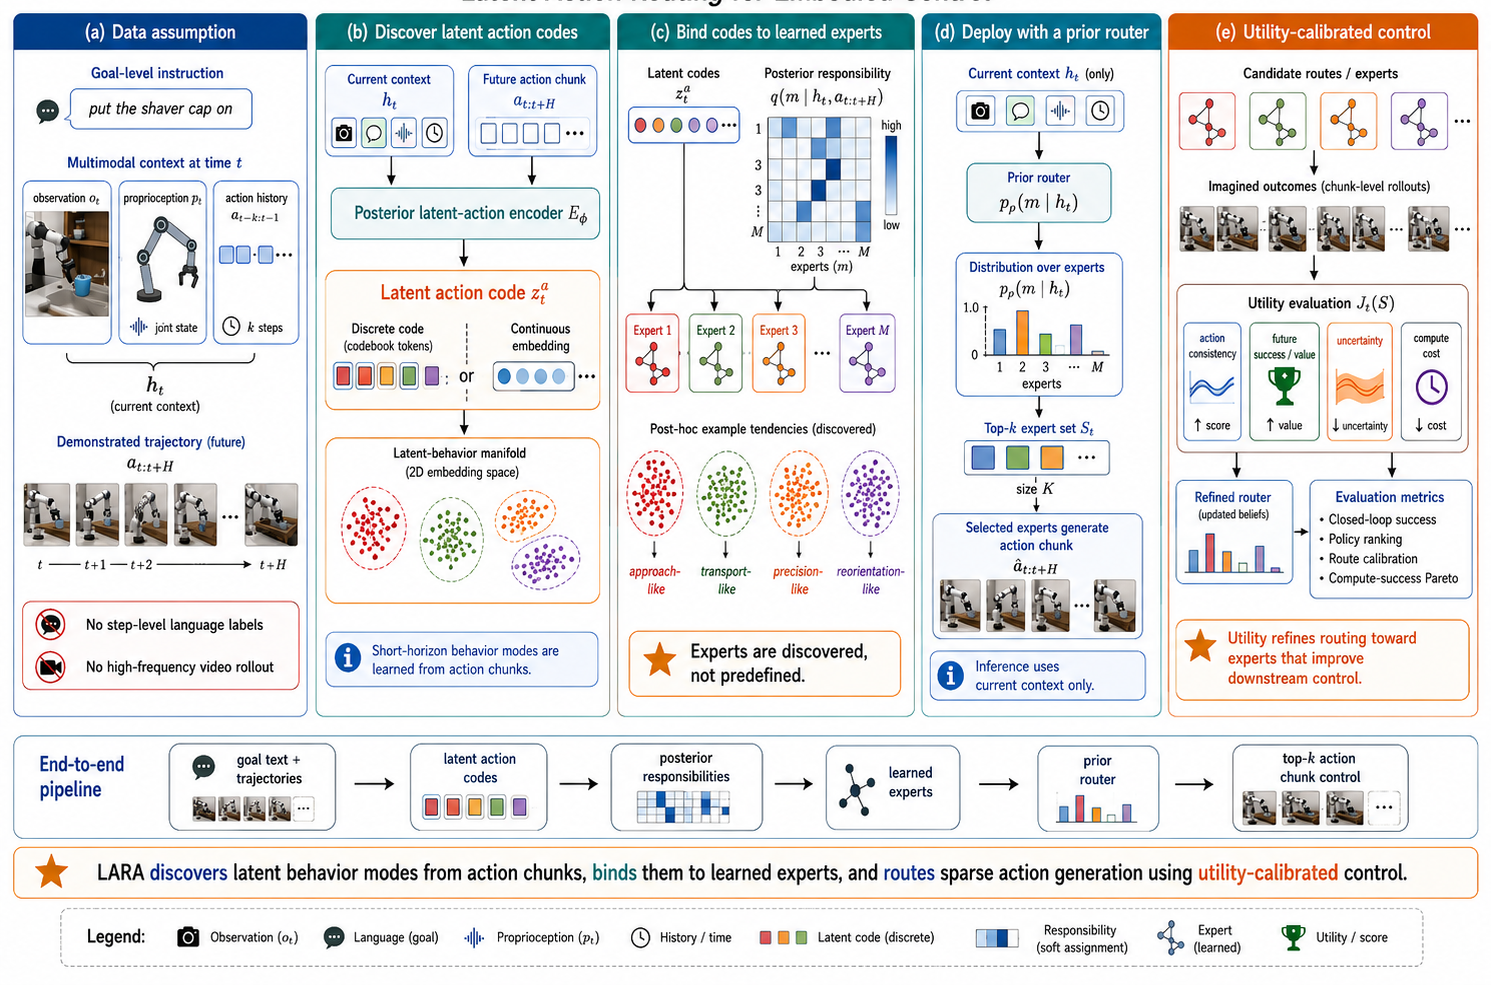
\includegraphics[width=\textwidth]{overview.png}
  \caption{Overview of LARA. Given ordinary goal-level language and robot demonstrations, LARA first discovers latent action codes from demonstrated future action chunks, without dense step-level language labels. The codes organize demonstrations into a latent behavior manifold and are softly bound to learned MoE action experts by posterior responsibility. A deployable router then predicts sparse expert selection from the current multimodal context alone. In deployment-oriented settings, this router can be two-level: an episode-level pool router selects a resident expert subset, while a chunk-level router selects top-$k$ experts inside the pool. Counterfactual utility fine-tuning calibrates routing toward experts that improve chunk-level control under matched active inference compute. Expert semantics are discovered post-hoc rather than manually predefined, and the method avoids high-frequency visual rollout generation.}
  \label{fig:overview}
\end{figure}

\section{Introduction}

Robot manipulation is usually specified at the level of intention. A person says, ``put the cap on the shaver'' or ``place the cup on the shelf,'' while the body produces a sequence of short motor behaviors without verbalizing every intermediate muscle contraction, contact transition, and corrective adjustment. This observation suggests a different way to build routed VLA systems. Rather than predefining experts as semantic, spatial, contact, articulation, or recovery modules, the model should discover behavior modes from trajectories and learn when each mode is useful for control.

A tempting design is to divide experts according to human-interpretable stages. That design is easy to explain, but it risks imposing an external taxonomy that the policy itself should not need. LARA instead takes the action chunk as the unit of discovery. Given the current multimodal context and a demonstrated future chunk, a posterior encoder infers a latent action code. Experts are then softly bound to regions of the learned behavior manifold by posterior responsibility. Their semantics are not fixed in advance; if an expert later appears approach-like, transport-like, or precision-like, that description is a post-hoc interpretation of the learned routing structure.

The central hypothesis is:
\begin{quote}
Robot demonstrations contain latent short-horizon behavior modes. If these modes are discovered from action chunks, softly bound to MoE experts by posterior responsibility, and routed at deployment by a context-only router calibrated with downstream control utility, then a VLA policy can use conditional capacity more effectively under a fixed active compute budget.
\end{quote}

This is not a claim that MoE removes dependence on data coverage or hardware constraints. Generalization remains bounded by the diversity and quality of robot data, and inference remains bounded by the deployable compute budget. The claim is instead about \emph{control generalization efficiency}: for the same goal-level text, trajectory data, active inference compute, and resident-expert budget, can a latent-action MoE policy reduce behavioral mode interference and improve closed-loop control?

\paragraph{Contributions.}
\begin{enumerate}
  \item We formulate VLA expert routing around \emph{latent action codes} learned from demonstrated action chunks, not human-defined manipulation stages or dense step-level text annotations.
  \item We propose a likelihood-based posterior responsibility mechanism that softly binds demonstrations and latent action codes to learned MoE action experts.
  \item We train a deployable router by distilling posterior expert responsibilities into a context-only route predictor, optionally factorized into an episode-level pool router and a chunk-level top-$k$ router for resident-expert efficiency.
  \item We refine routing with counterfactual control utility, so experts are selected for downstream control value rather than only demonstration reconstruction.
  \item We define a matched-compute and matched-resident-expert experimental protocol that tests closed-loop success, policy ranking, route calibration, subset retention, and compute-success Pareto efficiency without high-frequency visual generation.
\end{enumerate}

\section{Related Work and Design Boundary}

\paragraph{Action-chunk policies and VLA control.}
Modern robot policies increasingly predict short action chunks rather than individual motor commands, as in diffusion-style visuomotor policies and action-chunking transformer policies \cite{chi2023diffusion}. LARA follows this chunked-control view: a goal-level instruction conditions a sequence of short-horizon behaviors, and the policy should discover the latent action modes that explain those behaviors. LARA is also compatible with larger VLA backbones such as RT-style policies, OpenVLA, or Octo-like generalist policies \cite{brohan2022rt1,brohan2023rt2,openvla2024,octo2024}, but the core claim is not tied to a specific large VLA implementation.

\paragraph{Sparse MoE and expert specialization.}
Sparse MoE models activate only a subset of experts per input, enabling conditional computation and larger total capacity at a fixed active compute budget \cite{shazeer2017moe,fedus2022switch}. However, generic MoE routing does not guarantee useful modularity. Experts may specialize according to low-level or unstable patterns, collapse to a few dominant modules, or fail to remain useful when subsets are deployed independently. Recent language-model MoE work on emergent modularity shows that subset usability should be designed and evaluated directly, rather than assumed from sparsity alone \cite{wang2026emo}. LARA incorporates the same engineering principle at the level of robot trajectories and action chunks: sparsity is useful only if the selected experts remain coherent and deployable under resident-memory budgets.

\paragraph{World models without dense video rollout.}
World models for control show the value of predicting future latent states for planning or policy improvement \cite{hafner2023dreamer,hansen2024tdmpc2}. LARA narrows this idea to chunk-level control. It does not require generating every intermediate visual frame. Instead, the optional transition target predicts a chunk-boundary latent state that is sufficient for the next decision step. This preserves control-relevant future supervision while avoiding high-frequency video generation.

\section{Problem Setup}

We assume a dataset of robot demonstrations
\begin{equation}
\mathcal{D}=\{\tau_i\}_{i=1}^{N}, \qquad
\tau_i=(g_i,o^i_{1:T_i},p^i_{1:T_i},a^i_{1:T_i}),
\label{eq:data}
\end{equation}
where $o_t$ is an observation such as RGB or multi-view RGB, $p_t$ is proprioception, $a_t$ is a robot action, and $g$ is a goal-level language instruction. The key data assumption is intentionally weak: $g$ is an ordinary task description such as ``put the shaver cap on,'' not a dense list of step-by-step action labels. Intermediate behavioral structure is expected to be learned from trajectories rather than specified by language annotations.

Some benchmarks additionally provide sparse rewards, success indicators, or termination annotations. We denote such optional signals by
\begin{equation}
\mathcal{Y}_\tau=\{r_{1:T},y_\tau,\delta_{1:T}\}
\end{equation}
when available, where $r_t$ is a reward, $y_\tau$ is an episode-level success label, and $\delta_t$ is an optional termination indicator. These signals are not required for latent-action discovery, expert binding, or prior-router distillation; they are used only for evaluation, optional value/progress heads, or utility calibration.

A multimodal encoder maps the current context to a control state
\begin{equation}
 h_t = F_\theta(o_t,g,p_t,a_{t-k:t-1}).
 \label{eq:context}
\end{equation}
The model predicts or reconstructs a short action chunk
\begin{equation}
 a_{t:t+H-1}=(a_t,a_{t+1},\ldots,a_{t+H-1}),
 \label{eq:chunk}
\end{equation}
rather than only a single action. Chunked control matters because a high-level intention is rarely expressed by one motor command; it is expressed by a short behavior sequence. Near the end of an episode, chunks that exceed the trajectory boundary are either omitted or evaluated with a valid-step mask.

In deployment we distinguish the \emph{prediction horizon} $H_p$ from the
\emph{execution horizon} $H_e$. The policy may predict a long future chunk
$\hat{a}_{t:t+H_p-1}$, while the controller executes only the first
$H_e$ actions before taking a new real observation and replanning. For the
SO101 setting considered here, the default 30Hz configuration is
\begin{equation}
H_p=60,\qquad H_e=10.
\label{eq:hp_he}
\end{equation}
Thus each policy call predicts two seconds of future actions, but only the
first one third of a second is actually sent to the robot before the next
closed-loop update.

We also allow a chunk-level state transition target. Instead of generating every intermediate image frame, the model predicts a control-sufficient future latent state at the chunk boundary,
\begin{equation}
\hat{h}_{t+H}=T_\psi(h_t,z_t^a),
\label{eq:transition}
\end{equation}
where $z_t^a$ is the latent action code introduced in the next section. The target state is obtained by encoding the real observation and proprioception at the chunk boundary,
\begin{equation}
\bar{h}_{t+H}=\bar{F}(o_{t+H},g,p_{t+H},a_{t+H-k:t+H-1}),
\label{eq:target_state}
\end{equation}
with $\bar{F}$ denoting a stop-gradient encoder or a slowly updated target encoder. This avoids the cost of high-frequency video generation while preserving supervision about where the system should be after executing the chunk.

With separate prediction and execution horizons, the transition objective can
supervise both the state at the next real replanning point and the longer
future structure:
\begin{equation}
\mathcal{L}_{\mathrm{state}} =
\lambda_{\mathrm{exec}}\|\hat{h}_{t+H_e}-\sg(\bar{h}_{t+H_e})\|_2^2
+\lambda_{\mathrm{pred}}\|\hat{h}_{t+H_p}-\sg(\bar{h}_{t+H_p})\|_2^2.
\label{eq:dual_horizon_state_loss}
\end{equation}
The $H_e$ term is the closed-loop term: it corresponds to the state at which
the robot will re-observe and replan. The $H_p$ term is an auxiliary long-range
target that encourages the latent action to preserve future structure beyond
the immediately executed segment.

\section{Learning Latent Action Codes}

\subsection{Posterior Latent-Action Encoder}

During training, the demonstrated future action chunk is known. A posterior latent-action encoder can therefore infer a compact behavior representation from the current context and the demonstrated chunk:
\begin{equation}
 e_t = E_\phi(h_t,a_{t:t+H-1}).
 \label{eq:posterior_embedding}
\end{equation}
The embedding $e_t$ is then converted into a latent action $z_t^a$, either by vector quantization in the discrete variant or by sampling from a conditional latent distribution in the continuous variant. Given $z_t^a$, the action-chunk decoder reconstructs the demonstrated chunk:
\begin{equation}
 \hat{a}_{t:t+H-1}=D_\theta(h_t,z_t^a).
 \label{eq:decode_chunk}
\end{equation}
For a deterministic decoder, the reconstruction loss is
\begin{equation}
 \mathcal{L}_{\mathrm{chunk}} = \|a_{t:t+H-1}-\hat{a}_{t:t+H-1}\|_2^2.
 \label{eq:chunk_loss}
\end{equation}
For a diffusion-style decoder, $D_\theta$ is replaced by an action denoiser conditioned on $(h_t,z_t^a)$, and the training loss is the standard denoising prediction objective.

\subsection{Discrete or Continuous Latent Action Codes}

The latent action $z_t^a$ can be represented either as a discrete codebook entry or as a continuous latent vector. In the discrete variant, the posterior encoder first maps the demonstrated chunk to the continuous embedding in Eq.~\ref{eq:posterior_embedding}. Given a learnable codebook $C=\{c_1,\ldots,c_K\}$, the embedding is quantized to its nearest code,
\begin{equation}
 k^\star=\arg\min_k \|e_t-c_k\|_2^2,\qquad z_t^a=c_{k^\star}.
 \label{eq:vq_quantize}
\end{equation}
The resulting code is used by the action-chunk decoder in Eq.~\ref{eq:decode_chunk}. The VQ objective is
\begin{equation}
\mathcal{L}_{\mathrm{VQ}}=
\mathcal{L}_{\mathrm{chunk}}
+\|\sg(e_t)-z_t^a\|_2^2
+\beta_{\mathrm{com}}\|e_t-\sg(z_t^a)\|_2^2,
\label{eq:vq_loss}
\end{equation}
where $\sg(\cdot)$ denotes stop-gradient. The first additional term updates the codebook, while the second is a commitment loss that encourages the posterior embedding to stay close to its selected code. We use a straight-through estimator for the quantized code so that decoder gradients are copied to the posterior embedding $e_t$.

Because the posterior encoder uses the future action chunk, it is not available at deployment. We therefore train a context-only latent-action prior
\begin{equation}
 p_\zeta(k|h_t)
 \label{eq:code_prior}
\end{equation}
over codebook entries. The discrete prior is trained to predict the posterior code assignment,
\begin{equation}
\mathcal{L}_{\mathrm{code\mbox{-}prior}}=CE(k^\star,p_\zeta(\cdot|h_t)),
\label{eq:code_prior_loss}
\end{equation}
where $k^\star$ is treated as a stop-gradient target. At inference time, the model samples or selects a latent action code from $p_\zeta(k|h_t)$ and decodes an action chunk without observing $a_{t:t+H-1}$. We monitor codebook perplexity and optionally use a code-usage regularizer to prevent collapse to a small number of codes.

A continuous variant can instead use a conditional variational encoder,
\begin{equation}
q_\phi(z_t^a|h_t,a_{t:t+H-1})=\mathcal{N}(\mu_\phi,\Sigma_\phi),
\label{eq:continuous_latent}
\end{equation}
with a learned context-only prior $p_\zeta(z_t^a|h_t)$. The prior is trained with
\begin{equation}
\mathcal{L}_{\mathrm{latent\mbox{-}prior}}=
\KL\left(q_\phi(z_t^a|h_t,a_{t:t+H-1})\,\|\,p_\zeta(z_t^a|h_t)\right).
\label{eq:latent_prior_loss}
\end{equation}
The discrete version is easier to visualize and analyze as an action-token vocabulary, while the continuous version can provide smoother interpolation for continuous control.

\subsection{Chunk-Level Future State Prediction}

The framework does not require high-frequency visual rollout generation. Instead of predicting every intermediate image frame $\hat{o}_{t+1:t+H}$, we predict only the chunk-boundary control state. A lightweight transition head predicts this boundary state from the current state and latent action:
\begin{equation}
\hat{h}_{t+H}=T_\psi(h_t,z_t^a).
\end{equation}
When a single chunk horizon is used, the state prediction loss is
\begin{equation}
\mathcal{L}_{\mathrm{state}}=\|T_\psi(h_t,z_t^a)-\sg(\bar{h}_{t+H})\|_2^2.
\label{eq:state_loss}
\end{equation}
In the receding-horizon variant, Eq.~\ref{eq:dual_horizon_state_loss} replaces
this single-boundary loss. A contrastive variant can replace either squared
term by pulling the predicted latent state toward the true boundary state and
pushing it away from negative boundary states from other chunks. This objective
makes the latent action useful not only for reconstructing the demonstrated
action chunk, but also for predicting where the system will be at the next
closed-loop replanning point and at the longer prediction boundary. For a pure
imitation variant, the transition head is optional; for the full
utility-calibrated LARA model, we include it by default because it provides the
main chunk-level predictive substrate for scoring candidate experts and routes.

\begin{figure}[t]
  \centering
  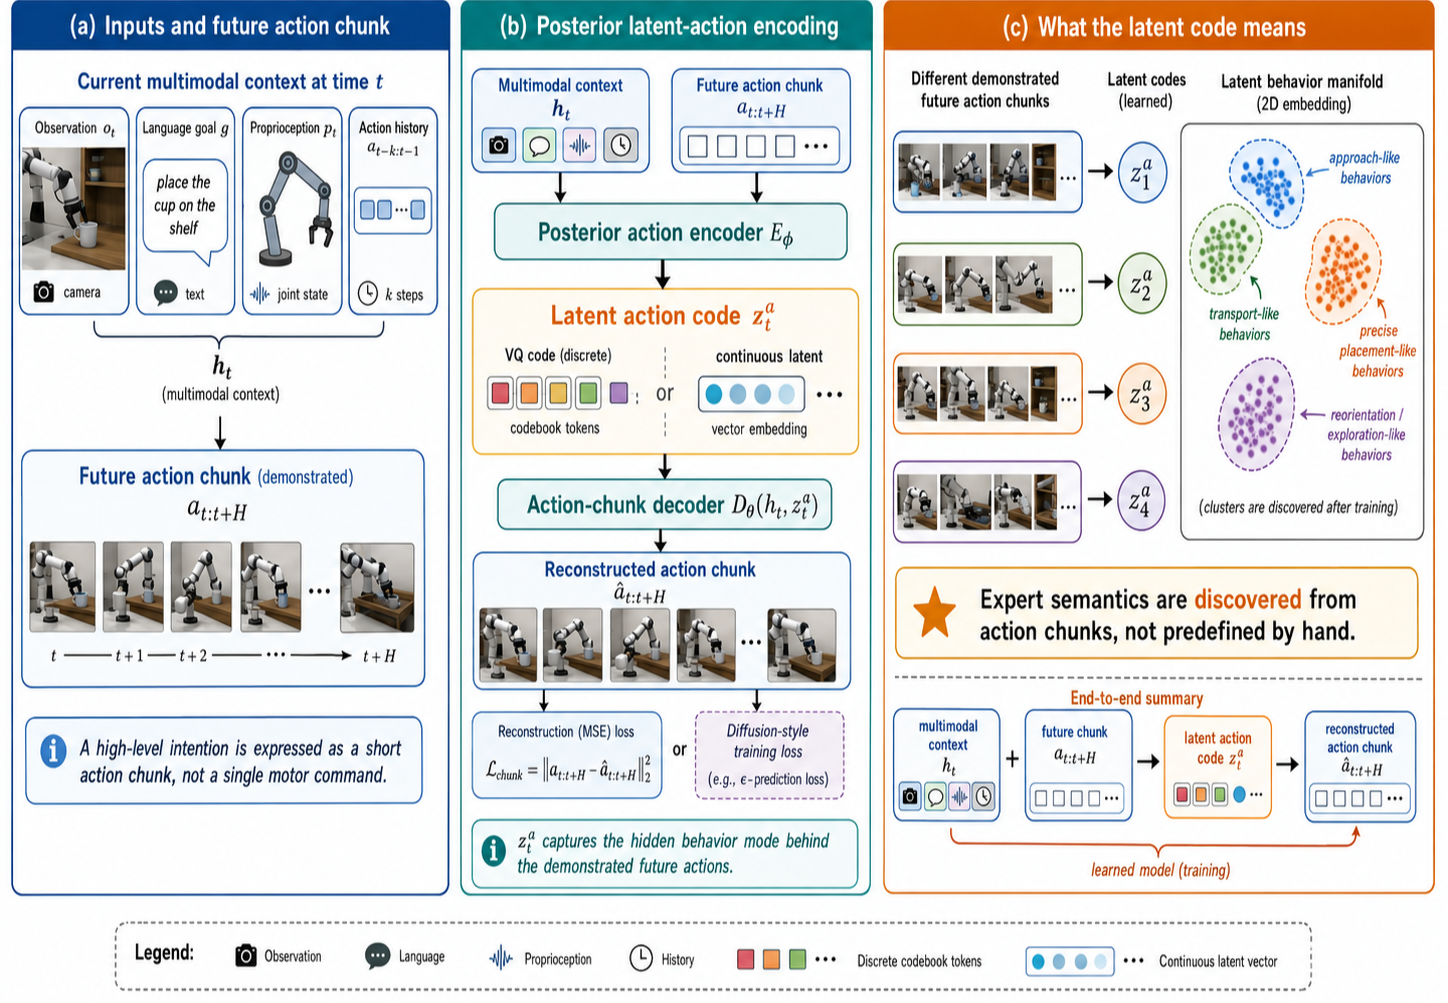
\includegraphics[width=\textwidth]{1.png}
  \caption{Learning latent action codes. A posterior action encoder observes the current multimodal context and a demonstrated future action chunk, then compresses the chunk into a latent action code. The code may be discrete, as in a VQ codebook, or continuous. It is trained to reconstruct the action chunk and to organize demonstrations into a latent behavior manifold.}
  \label{fig:latent_action}
\end{figure}

\section{Binding Latent Action Codes to MoE Experts}

Let there be $M$ expert action generators $\{E_m\}_{m=1}^M$. Expert $m$ defines a likelihood or reconstruction score for a demonstrated chunk:
\begin{equation}
 p_m(a_{t:t+H-1}|h_t) \quad \text{or} \quad \ell_m(a_{t:t+H-1};h_t).
\end{equation}
The posterior responsibility of expert $m$ for a demonstrated chunk is
\begin{equation}
 q(m|h_t,a_{t:t+H-1}) =
 \frac{\exp(-\ell_m(a_{t:t+H-1};h_t)/\tau_q)}
 {\sum_{j=1}^{M}\exp(-\ell_j(a_{t:t+H-1};h_t)/\tau_q)},
 \label{eq:responsibility}
\end{equation}
or equivalently $q(m|h_t,a_{t:t+H-1})\propto p(a_{t:t+H-1}|h_t,m)$.

The expert loss is responsibility-weighted:
\begin{equation}
 \mathcal{L}_{\mathrm{expert}} =
 \sum_{i\in\mathcal{B}}\sum_{m=1}^{M}
 q(m|h_i,a_{i:i+H-1})\,\ell_m(a_{i:i+H-1};h_i).
 \label{eq:expert_loss}
\end{equation}
This is a soft assignment, not a hard split of the dataset. A demonstration can update multiple experts, but it updates most strongly the experts that explain it best. The mechanism resembles soft EM: responsibilities estimate which expert explains which region of the behavior manifold, and the experts improve on the demonstrations for which they have high responsibility.

This design avoids a hand-coded taxonomy. We do not say that Expert 1 is contact, Expert 2 is transport, or Expert 3 is recovery. If such tendencies appear after training, they are post-hoc interpretations of learned behavior regions, not imposed labels.

\begin{figure}[t]
  \centering
  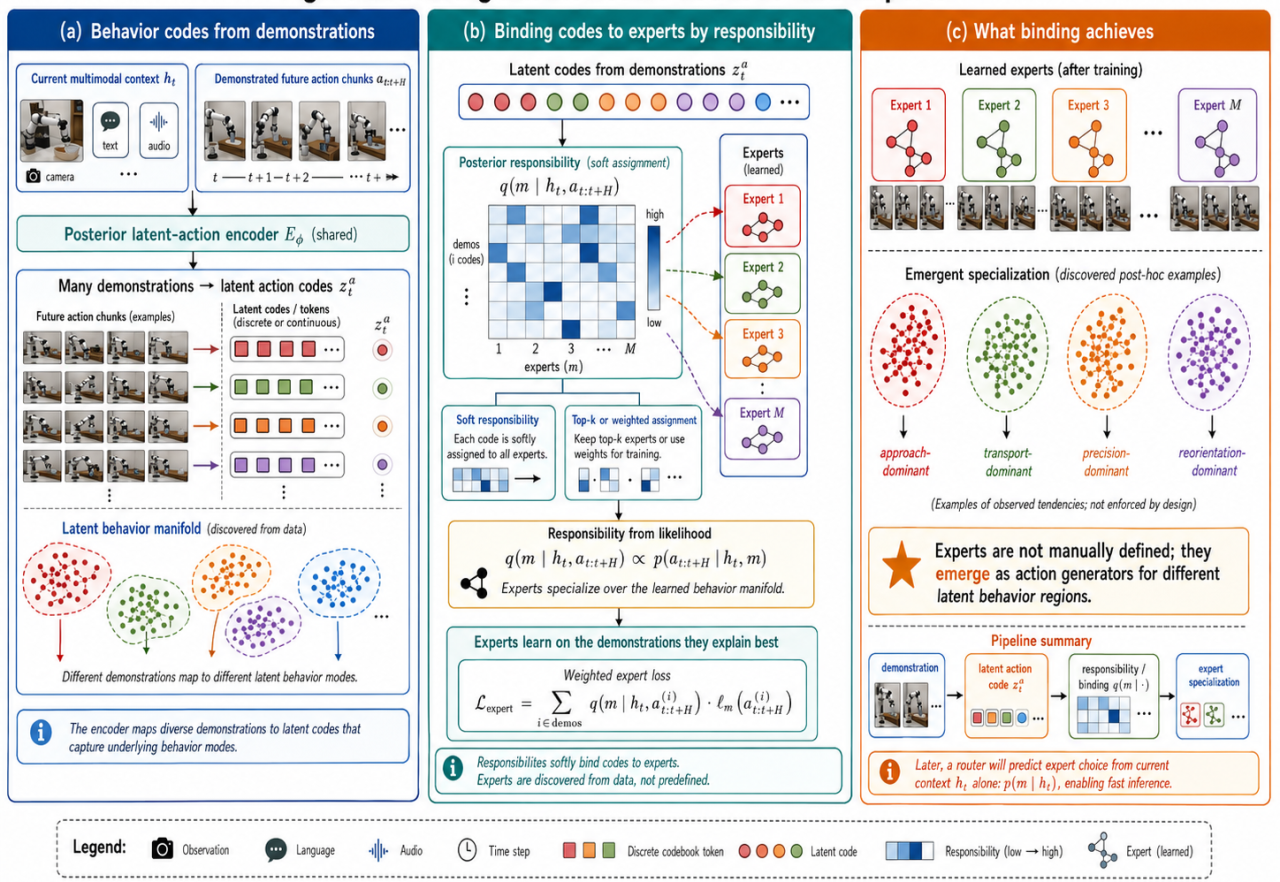
\includegraphics[width=\textwidth]{2.png}
  \caption{Binding latent action codes to MoE experts. Demonstrations are encoded into latent action codes, then softly assigned to learned experts by posterior responsibility. Experts are not manually named or predefined; they emerge as action generators for different regions of the latent behavior manifold.}
  \label{fig:binding}
\end{figure}

\section{Training the Router}

\subsection{Posterior Teacher}

The responsibility distribution in Eq.~\ref{eq:responsibility} is a training-time posterior signal because it depends on the demonstrated future action chunk. We denote it
\begin{equation}
 q_{\mathrm{post}}(m|h_t,a_{t:t+H-1}).
\end{equation}
It answers: \emph{which expert explains the demonstrated future behavior?}

\subsection{Episode-Level Pool Router}

For memory-constrained deployment, the route predictor can be factorized into two levels. At the beginning of an episode or task, an episode-level pool router chooses a resident expert pool
\begin{equation}
P_\tau=\TopD(p_\chi(m|g,h_1,b),d_\tau),
\label{eq:pool_router}
\end{equation}
where $h_1$ is the initial context, $g$ is the goal instruction, and $b$ is an optional deployment budget. The pool size $d_\tau$ can be fixed for a target device or sampled during training to support multiple resident-expert budgets. This makes routing not only sparse per chunk, but also localized over the episode: only experts in $P_\tau$ must be resident for that rollout.

During training, a natural posterior pool target is obtained by averaging posterior responsibilities over chunks in the trajectory:
\begin{equation}
\bar{q}_\tau(m)=\frac{1}{|\mathcal{T}_\tau|}\sum_{t\in\mathcal{T}_\tau}q_{\mathrm{post}}(m|h_t,a_{t:t+H-1}).
\end{equation}
The pool router can be trained by a masked distillation objective
\begin{equation}
\mathcal{L}_{\mathrm{pool}}=\KL\left(\sg(\bar{q}_\tau)\|p_\chi(\cdot|g,h_1,b)\right).
\end{equation}
This pooling mechanism is an implementation choice, not a substitute for latent-action discovery. It should be ablated by reporting closed-loop success as a function of resident expert percentage. Similar subset-retention evaluation is used in modular MoE language modeling, where expert subsets are assessed directly under memory budgets \cite{wang2026emo}.

\subsection{Chunk-Level Prior Router}

At deployment, the future action chunk is unavailable. The chunk-level router must use only current context and, when enabled, must route within the episode pool. Define masked router logits
\begin{equation}
\tilde{r}_\rho^m(h_t,P_\tau)=
\begin{cases}
r_\rho^m(h_t), & m\in P_\tau,\\
-\infty, & m\notin P_\tau.
\end{cases}
\end{equation}
The masked route distribution is
\begin{equation}
 p_\rho(m|h_t,P_\tau)=\softmax(\tilde{r}_\rho(h_t,P_\tau))_m.
\end{equation}
Without an episode pool, $P_\tau$ is the full expert set. The active route is a sparse top-$k$ set
\begin{equation}
 S_t=\TopK(p_\rho(m|h_t,P_\tau),k),\quad S_t\subseteq P_\tau.
\end{equation}
with normalized weights over selected experts. The action generator is
\begin{equation}
 \hat{a}_{t:t+H-1}=\sum_{m\in S_t} \omega_t^m E_m(h_t), \quad
 \omega_t^m=\frac{\exp(r_\rho^m(h_t)/\tau_r)}{\sum_{j\in S_t}\exp(r_\rho^j(h_t)/\tau_r)}.
\end{equation}

The chunk router is first trained by distilling the posterior teacher:
\begin{equation}
 \mathcal{L}_{\mathrm{distill}} =
 \KL\left(\sg(q_{\mathrm{post}}(\cdot|h_t,a_{t:t+H-1}))\|p_\rho(\cdot|h_t,P_\tau)\right).
 \label{eq:distill}
\end{equation}
Load balancing and route stickiness regularize this phase:
\begin{equation}
 \mathcal{L}_{\mathrm{stick}}=\|p_\rho(\cdot|h_t,P_\tau)-p_\rho(\cdot|h_{t-1},P_\tau)\|_1.
\end{equation}

Load balancing should be measured across a sufficiently diverse batch of episodes, not forced within a single episode where pool consistency is desired. Stickiness prevents high-frequency route thrashing.

\begin{figure}[t]
  \centering
  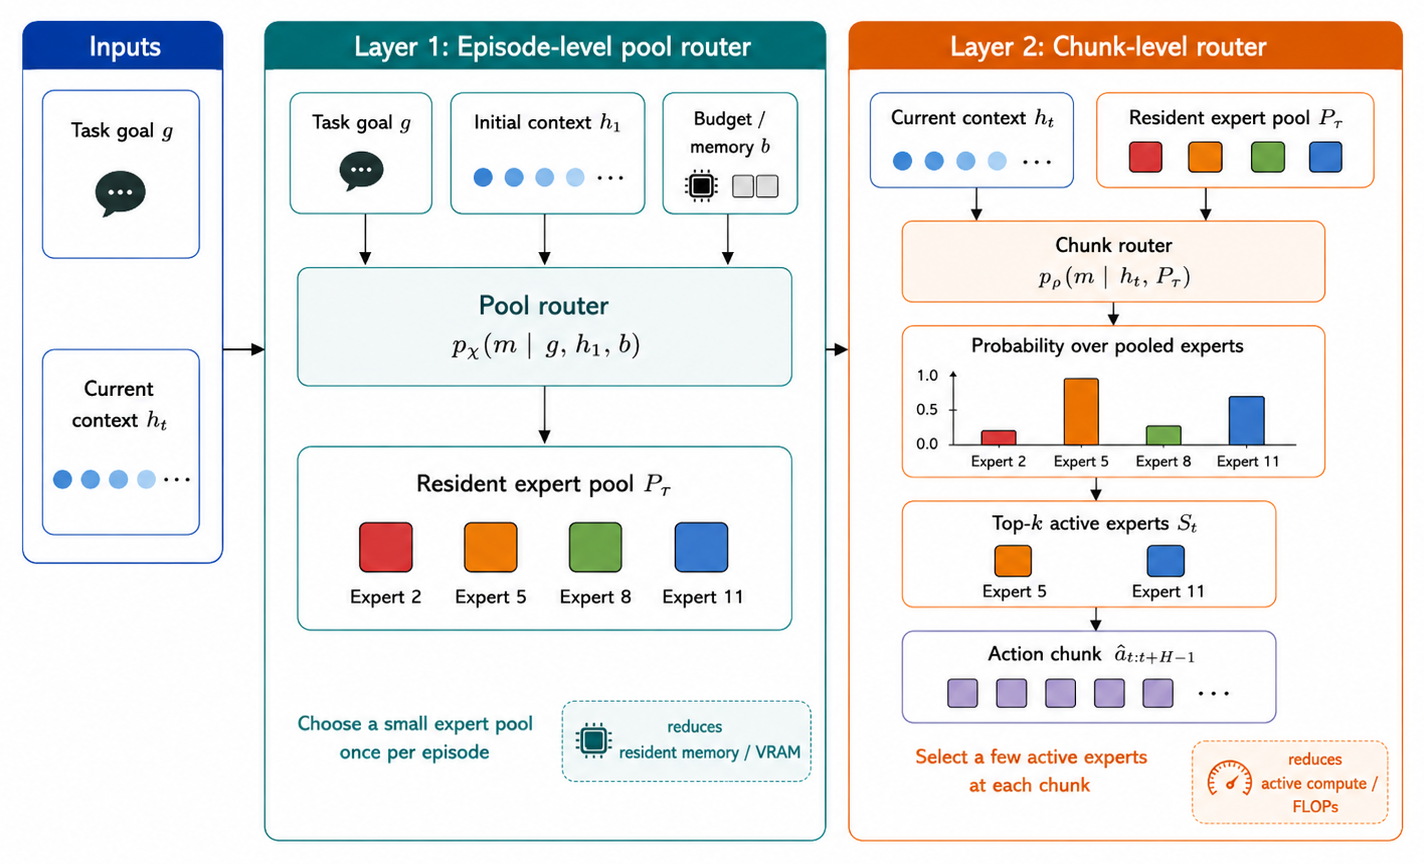
\includegraphics[width=\textwidth]{3.png}
  \caption{Two-level router for deployment-oriented sparse action generation. The episode-level pool router selects a small resident expert pool $P_\tau$ once per task from the goal, initial context, and device budget, reducing resident memory. The chunk-level router then selects a top-$k$ active set $S_t\subseteq P_\tau$ from the current context at each control step, reducing active compute while preserving local flexibility.}
  \label{fig:dual_router}
\end{figure}

\subsection{Counterfactual Utility Fine-Tuning}

Reconstructing demonstrations is not the same as improving control. The final router objective therefore evaluates candidate experts or routes by a downstream control utility. For a candidate route $S$ at context $h_t$, define
\begin{align}
J_t(S)=&-\alpha\,\ell_{\mathrm{act}}(\hat{a}_{t:t+H-1}^{S},a_{t:t+H-1})
-\alpha_s\,d(\hat{h}_{t+H}^{S},\bar{h}_{t+H}) \nonumber\\
&+\beta\,V^{-}(\hat{h}_{t+H}^{S},g)
-\delta\,\sigma^{-}(\hat{h}_{t+H}^{S},g)
-\eta\,\Cost(S).
\label{eq:utility}
\end{align}
Here $V^{-}$ is a lagged value or progress predictor, $\sigma^{-}$ is an uncertainty or instability estimate, and $\Cost(S)$ is active inference cost. If sparse success or reward labels are available, $V^{-}$ may be trained as a success/value head; otherwise it can be replaced by proxy progress, latent-state consistency, or ranking signals. The key difference from video-world-model training is that utility is computed over action chunks and chunk-boundary latent states, not dense visual frame predictions.

For a candidate expert $m$ or route replacement $S_t(m)$, the centered utility target is
\begin{equation}
 U_t^m = J_t(S_t(m)) - \frac{1}{|\mathcal{C}_t|}\sum_{j\in\mathcal{C}_t}J_t(S_t(j)),
\end{equation}
where $\mathcal{C}_t$ is a small candidate set consisting of the current route and sampled alternatives. The utility regression loss is
\begin{equation}
 \mathcal{L}_{\mathrm{utility}} =
 \frac{1}{|\mathcal{C}_t|}\sum_{m\in\mathcal{C}_t}
 \operatorname{Huber}(r_\rho^m(h_t),\sg(U_t^m)).
 \label{eq:utility_loss}
\end{equation}
A pairwise ranking loss can be added to improve top-$k$ ordering:
\begin{equation}
\mathcal{L}_{\mathrm{rank}}=\mathbb{E}_{i,j}\log\left(1+\exp[-\sg(U_t^i-U_t^j)(r_\rho^i(h_t)-r_\rho^j(h_t))]\right).
\end{equation}

\subsection{Collapse Prevention and Routing Stabilization}

Sparse latent-action routing can fail by collapsing to a small set of codes, experts, or routes. We therefore stabilize training at several levels rather than relying on load balancing alone.

\paragraph{Latent-code usage.}
For the discrete variant, we monitor the code usage distribution $\bar{p}_{\mathrm{code}}(k)$ and its perplexity,
\begin{equation}
\operatorname{PPL}_{\mathrm{code}}=
\exp\left(-\sum_{k=1}^{K}\bar{p}_{\mathrm{code}}(k)\log \bar{p}_{\mathrm{code}}(k)\right).
\end{equation}
Low perplexity or a high dead-code ratio indicates codebook collapse. We optionally add a weak code-usage regularizer
\begin{equation}
\mathcal{L}_{\mathrm{code\mbox{-}bal}}
=\KL\left(\mathbf{u}_K\,\|\,\bar{p}_{\mathrm{code}}\right),
\end{equation}
where $\mathbf{u}_K$ is the uniform distribution over codebook entries. In implementation, EMA codebook updates or dead-code reinitialization can be used when many codes remain unused for long intervals.

\paragraph{Responsibility smoothing.}
Expert specialization is driven by $q_{\mathrm{post}}$. If the responsibility distribution becomes too sharp early in training, a slightly better expert can absorb most chunks before other experts learn. We therefore use a high initial temperature $\tau_q$ and anneal it only after the experts begin to specialize. We also allow a small uniform floor,
\begin{equation}
\tilde{q}_{\mathrm{post}}(m|h_t,\achunk)
=(1-\epsilon)q_{\mathrm{post}}(m|h_t,\achunk)+\epsilon/M,
\end{equation}
or a top-$r$ soft assignment that updates several high-responsibility experts instead of using a hard top-1 assignment. These choices give non-dominant experts gradient signal during early training.

\paragraph{Expert and router balance.}
For chunk-level routing, balancing should be measured across a diverse batch of episodes rather than inside a single episode. For episode-level pools, balancing is likewise computed over many trajectories. A generic form is
\begin{equation}
\mathcal{L}_{\mathrm{lb}}
=\KL(\mathbf{u}_M\,\|\,\bar{p}_{\mathrm{route}})
+\KL(\mathbf{u}_M\,\|\,\bar{p}_{\mathrm{pool}}),
\end{equation}
where $\bar{p}_{\mathrm{route}}$ is the average chunk-level route distribution and $\bar{p}_{\mathrm{pool}}$ is the average episode-level pool distribution. Early training can also use router entropy regularization or noisy top-$k$ routing to encourage exploration. Route stickiness is kept as a separate stabilizer because it prevents high-frequency route thrashing without forcing all experts to be used inside one trajectory.

\paragraph{Expert diversity and capacity.}
Balanced usage does not guarantee distinct expert functions. We monitor pairwise similarity of expert outputs on shared inputs and optionally add a weak decorrelation penalty,
\begin{equation}
\mathcal{L}_{\mathrm{div}}
=\frac{1}{M(M-1)}\sum_{m\ne n}
\left(\frac{E_m(u_t)^\top E_n(u_t)}{\|E_m(u_t)\|\,\|E_n(u_t)\|}\right)^2,
\quad u_t=[h_t,z_t^a].
\end{equation}
Expert dropout or soft capacity limits can further prevent early dominant experts from consuming most high-responsibility chunks.

\paragraph{Delayed utility calibration.}
Counterfactual utility should not dominate before the latent codes, experts, and prior router are reasonably stable. We therefore start with latent-action reconstruction and posterior-responsibility training, then add prior-router distillation, and only later increase the weight of $\mathcal{L}_{\mathrm{utility}}$. Utility targets use stop-gradient labels and lagged value or uncertainty heads. We retain a nonzero distillation weight during utility fine-tuning so that routing remains close to the demonstrated behavior distribution while being calibrated toward downstream control.

We collect optional stabilization terms as
\begin{equation}
\mathcal{L}_{\mathrm{stab}}
=\lambda_{\mathrm{code}}\mathcal{L}_{\mathrm{code\mbox{-}bal}}
+\lambda_{\mathrm{div}}\mathcal{L}_{\mathrm{div}}
+\lambda_{\mathrm{ent}}\mathcal{L}_{\mathrm{ent}},
\end{equation}
where $\mathcal{L}_{\mathrm{ent}}$ denotes an early-stage router-entropy term. These terms are treated as training stabilizers and should be ablated separately from the core latent-action and utility-routing claims.

\section{Full Objective and Algorithm}

The full training objective is
\begin{align}
\mathcal{L}=&\mathcal{L}_{\mathrm{chunk}}
+\lambda_z\mathcal{L}_{\mathrm{latent}}
+\lambda_s\mathcal{L}_{\mathrm{state}}
+\lambda_e\mathcal{L}_{\mathrm{expert}}
+\lambda_p\mathcal{L}_{\mathrm{pool}}
+\lambda_d\mathcal{L}_{\mathrm{distill}} \nonumber\\
&+\lambda_u\mathcal{L}_{\mathrm{utility}}
+\lambda_r\mathcal{L}_{\mathrm{rank}}
+\lambda_{\mathrm{lb}}\mathcal{L}_{\mathrm{lb}}
+\lambda_{\mathrm{st}}\mathcal{L}_{\mathrm{stick}}
+\lambda_{\mathrm{stab}}\mathcal{L}_{\mathrm{stab}}.
\label{eq:full_objective}
\end{align}
The latent regularizer $\mathcal{L}_{\mathrm{latent}}$ contains the codebook, commitment, and code-prior terms for the discrete variant, or the variational prior KL for the continuous variant. The reconstruction term $\mathcal{L}_{\mathrm{chunk}}$ is written separately to avoid double counting. If the episode pool is not used, $\lambda_p=0$ and $P_\tau$ is the full expert set.

\begin{algorithm}[H]
\caption{Training Latent-Action Routing}
\begin{algorithmic}[1]
\State Sample demonstration chunks $(o_t,g,p_t,a_{t-k:t-1},a_{t:t+H_p-1},o_{t+H_e},p_{t+H_e},o_{t+H_p},p_{t+H_p})$.
\State Encode current and boundary states: $h_t=F_\theta(o_t,g,p_t,a_{t-k:t-1})$, $\bar{h}_{t+H_e}=\bar{F}(o_{t+H_e},g,p_{t+H_e},a_{t+H_e-k:t+H_e-1})$, and $\bar{h}_{t+H_p}=\bar{F}(o_{t+H_p},g,p_{t+H_p},a_{t+H_p-k:t+H_p-1})$.
\State Infer posterior latent action embedding $e_t=E_\phi(h_t,a_{t:t+H_p-1})$ and obtain $z_t^a$ by quantization or continuous sampling.
\State Train action decoder and chunk-boundary transition with $\mathcal{L}_{\mathrm{chunk}}$ and $\mathcal{L}_{\mathrm{state}}$.
\State Compute posterior expert responsibilities $q_{\mathrm{post}}(m|h_t,a_{t:t+H_p-1})$.
\State Update experts with responsibility-weighted loss $\mathcal{L}_{\mathrm{expert}}$.
\State Optionally aggregate responsibilities over the episode and train $p_\chi(P_\tau|g,h_1,b)$ with $\mathcal{L}_{\mathrm{pool}}$.
\State Train the chunk-level prior router $p_\rho(m|h_t,P_\tau)$ by distillation from $q_{\mathrm{post}}$.
\State Apply stabilization terms, including code-usage monitoring, smoothed responsibilities, global load balancing, route stickiness, and optional expert-diversity regularization.
\State After warm-up, evaluate a small set of candidate routes using $J_t(S)$ and train router scores with $\mathcal{L}_{\mathrm{utility}}$ and $\mathcal{L}_{\mathrm{rank}}$.
\end{algorithmic}
\end{algorithm}

At inference time, the system executes only the context encoder, deployable router, selected experts, and action decoder:
\begin{equation}
 (g,h_1,b)\rightarrow P_\tau,\qquad h_t\rightarrow S_t\subseteq P_\tau\rightarrow \hat{a}_{t:t+H_p-1}.
\end{equation}
Only the prefix $\hat{a}_{t:t+H_e-1}$ is executed. The next policy call starts
from the real observation and proprioception at $t+H_e$, not from a predicted
latent state:
\begin{equation}
o_{t+H_e},p_{t+H_e}\rightarrow h_{t+H_e}\rightarrow
\hat{a}_{t+H_e:t+H_e+H_p-1}.
\end{equation}
If the episode pool is disabled, $P_\tau$ is the full expert set. The posterior
action encoder, future-action teacher, and counterfactual candidate scoring are
training-time mechanisms. Predicted latent states are used for training and
utility calibration, not as the next round's real closed-loop input.

\subsection*{Current Repository Implementation Status}

The current repository implements only the SO101 VLA-JEPA action baseline: the
pretrained VLA representation is reused, latent and embodied action tokens are
extracted from the token stream, and a flow-matching action head predicts the
continuous follower-arm action chunk. This is not yet the full LARA algorithm in
this manuscript. In particular, production-ready latent-action training, MoE
action experts, posterior responsibility training, the episode-level pool
router, the chunk-level top-$k$ router inside the resident pool, and
counterfactual utility calibration remain future implementation work. Any
current latent-action or MoE/router code should be treated as disabled
experimental scaffolding until it has full training, diagnostic, and closed-loop
validation.

\section{Experimental Protocol}

\subsection{Data and Language Assumption}

The main protocol should use ordinary goal-level language and trajectories. No dense step-level language labels are required. Each episode contains
\begin{equation}
(g,o_{1:T},p_{1:T},a_{1:T}).
\end{equation}
Optional signals such as sparse reward $r_t$, episode success $y_\tau$, or termination annotations $\delta_t$ may be recorded by a benchmark, simulator, or external evaluator, but the primary representation-learning pipeline does not require them. Trajectory boundaries are handled as data boundaries: chunks that extend beyond the recorded trajectory are masked out of the reconstruction and transition losses. A recommended ablation compares: (i) goal-only language, (ii) goal plus terminal success condition when available, and (iii) dense step annotations. The primary method should not depend on (iii), and should report whether utility heads use true success labels or proxy progress signals.

\subsection{Benchmarks}

The minimal experimental stack is:
\begin{itemize}
  \item \textbf{ManiSkill3}: fast sanity checks and ablations over $M$, $k$, chunk horizon $H$, utility components, and route-pool budgets.
  \item \textbf{LIBERO}: language-conditioned manipulation and transfer splits.
  \item \textbf{CALVIN}: long-horizon multi-step manipulation.
\end{itemize}
A real-data ranking track, such as DROID, BridgeData V2, robomimic, or Open X-Embodiment subsets, can be added for policy-ranking and route-calibration analysis if compute allows.

\subsection{Baselines}

The primary causal baselines are:
\begin{enumerate}
  \item Dense VLA with the same backbone and action-chunk decoder.
  \item Generic sparse MoE-VLA with load balancing but no latent-action posterior responsibility.
  \item Latent-action MoE without utility fine-tuning.
  \item LARA without episode-level pool routing.
  \item LARA with two-level route-pool deployment.
  \item Dense-large with matched total parameters, when feasible.
  \item Dense-small with matched active parameters.
\end{enumerate}
All primary comparisons must report total parameters, resident parameters, active parameters, inference FLOPs, latency, and VRAM.

\subsection{Metrics}

The primary metric is closed-loop success under matched active inference compute. Secondary metrics are return, sample-efficiency AUC, compute-success Pareto efficiency, policy-ranking Spearman $\rho$ and Kendall $\tau$, top-$k$ route consistency, route regret, expert usage entropy, route-switch frequency, utility calibration error, train-time overhead, and inference latency. If the episode-level route pool is used, also report subset-retention curves: success versus percentage of resident experts retained, e.g., 100\%, 50\%, 25\%, and 12.5\% resident experts.

\begin{table}[t]
\centering
\caption{Primary matched-compute results. Entries are placeholders to be filled by completed runs.}
\label{tab:main}
\small
\begin{tabular}{llrrrrrr}
\toprule
Benchmark & Method & Success $\uparrow$ & Return $\uparrow$ & Resident Params $\downarrow$ & FLOPs $\downarrow$ & Latency $\downarrow$ & Route Regret $\downarrow$ \\
\midrule
LIBERO & Dense VLA & TBD & TBD & TBD & TBD & TBD & -- \\
LIBERO & Generic MoE & TBD & TBD & TBD & TBD & TBD & TBD \\
LIBERO & Latent-Action MoE & TBD & TBD & TBD & TBD & TBD & TBD \\
LIBERO & LARA & TBD & TBD & TBD & TBD & TBD & TBD \\
LIBERO & LARA + route pool & TBD & TBD & TBD & TBD & TBD & TBD \\
\midrule
CALVIN & Dense VLA & TBD & TBD & TBD & TBD & TBD & -- \\
CALVIN & Generic MoE & TBD & TBD & TBD & TBD & TBD & TBD \\
CALVIN & Latent-Action MoE & TBD & TBD & TBD & TBD & TBD & TBD \\
CALVIN & LARA & TBD & TBD & TBD & TBD & TBD & TBD \\
CALVIN & LARA + route pool & TBD & TBD & TBD & TBD & TBD & TBD \\
\bottomrule
\end{tabular}
\end{table}

\begin{table}[t]
\centering
\caption{Ablation plan for isolating the causal role of latent action discovery, expert binding, utility-calibrated routing, and deployment-oriented route-pool choices.}
\label{tab:ablation}
\small
\begin{tabular}{lllrr}
\toprule
Block & Variant & Question & Success $\uparrow$ & Rank $\rho$ $\uparrow$ \\
\midrule
Representation & No latent action code & Does chunk latent modeling matter? & TBD & TBD \\
Binding & Hard cluster assignment & Is soft responsibility needed? & TBD & TBD \\
Binding & Generic MoE only & Is the gain just sparsity? & TBD & TBD \\
Router & Distillation only & Is posterior-to-prior routing sufficient? & TBD & TBD \\
Router & Utility only & Does utility work without teacher warm-up? & TBD & TBD \\
Router & Full distill + utility & Does complete route calibration help? & TBD & TBD \\
Deployment & No episode pool & Does ordinary chunk routing suffice? & TBD & TBD \\
Deployment & Fixed pool size & Is a fixed resident budget brittle? & TBD & TBD \\
Deployment & Randomized pool size & Does budget randomization improve retention curves? & TBD & TBD \\
Language & Goal-only & Are step labels necessary? & TBD & TBD \\
Language & Goal + terminal condition & Does outcome text help? & TBD & TBD \\
Language & Dense step text & Does step supervision overfit routing? & TBD & TBD \\
\bottomrule
\end{tabular}
\end{table}

\subsection{Success and Failure Conditions}

The main claim should be accepted only if the full method improves closed-loop success over both Dense VLA and Generic MoE under matched active compute, and also improves at least one of policy-ranking fidelity, route calibration, or route regret. If it beats Dense VLA but not Generic MoE, the evidence supports sparsity but not latent-action responsibility or utility routing. If the route-pool variant improves resident-parameter efficiency but not control, the result should be framed as a deployment optimization rather than as the core learning claim.

\section{Discussion}

The revised framework changes the interpretation of experts. They are no longer hand-labeled manipulation phases. They are learned action generators tied to regions of a latent behavior manifold. This better matches the intuition that an embodied agent should reason at the level of goals and short-horizon behavior modes, not explicit per-step muscle-like instructions.

The framework also narrows the role of world modeling. It does not require dense visual prediction. For control, the useful prediction target can be a chunk-boundary latent state, a value or success estimate, and an uncertainty estimate. This makes the method more deployable than high-frequency video generation while preserving enough structure for counterfactual utility evaluation.

The two-level routing implementation connects active-compute efficiency with resident-memory efficiency. Chunk-level top-$k$ routing reduces activated computation, while the episode-level pool can reduce which experts need to be resident during a rollout. These benefits must be measured separately. A method may be FLOP-efficient but not VRAM-efficient if all experts remain resident, so the experimental protocol reports both active parameters and resident parameters.

\section{Limitations}

The method does not bypass data limitations. If the demonstrations do not cover the necessary behavior modes, latent-action discovery cannot invent them. MoE also does not automatically reduce VRAM: if all experts are resident on the device, memory may increase, even if active FLOPs decrease. Practical deployment should prefer shared VLA backbones with small MoE adapters or action heads. Finally, the posterior teacher can produce misleading responsibilities if the experts are weak early in training; curriculum, entropy regularization, warm-started dense action models, and explicit collapse diagnostics are likely necessary. Stabilizers such as load balancing or diversity penalties must be tuned carefully, since overly strong regularization can force artificial expert usage and degrade control performance.

\section{Conclusion}

We proposed LARA, Latent Action Routing for embodied VLA control. The method learns latent action codes from demonstrated action chunks, binds them to experts by posterior responsibility, distills expert choice into a deployable router, and calibrates the router with counterfactual control utility. A deployment-oriented implementation can factor routing into episode-level resident expert selection and chunk-level top-$k$ activation. The resulting system uses ordinary goal-level language and trajectories, avoids hand-designed expert taxonomies, and avoids expensive dense visual rollout generation. Its empirical test is clear: under matched active compute and resident-expert budgets, it should improve closed-loop control and route quality relative to dense VLA and generic sparse MoE baselines.

\begin{thebibliography}{10}
\bibitem{shazeer2017moe}
Noam Shazeer et al.
\newblock Outrageously large neural networks: The sparsely-gated mixture-of-experts layer.
\newblock \emph{ICLR}, 2017.

\bibitem{fedus2022switch}
William Fedus, Barret Zoph, and Noam Shazeer.
\newblock Switch Transformers: Scaling to trillion parameter models with simple and efficient sparsity.
\newblock \emph{JMLR}, 2022.

\bibitem{chi2023diffusion}
Cheng Chi et al.
\newblock Diffusion Policy: Visuomotor policy learning via action diffusion.
\newblock \emph{RSS}, 2023.

\bibitem{brohan2022rt1}
Anthony Brohan et al.
\newblock RT-1: Robotics Transformer for real-world control at scale.
\newblock arXiv:2212.06817, 2022.

\bibitem{brohan2023rt2}
Anthony Brohan et al.
\newblock RT-2: Vision-language-action models transfer web knowledge to robotic control.
\newblock \emph{CoRL}, 2023.

\bibitem{openvla2024}
Moo Jin Kim et al.
\newblock OpenVLA: An open-source vision-language-action model.
\newblock arXiv:2406.09246, 2024.

\bibitem{octo2024}
Octo Model Team et al.
\newblock Octo: An open-source generalist robot policy.
\newblock arXiv:2405.12213, 2024.

\bibitem{hafner2023dreamer}
Danijar Hafner et al.
\newblock Mastering diverse domains through world models.
\newblock arXiv:2301.04104, 2023.

\bibitem{hansen2024tdmpc2}
Nicklas Hansen, Hao Su, and Xiaolong Wang.
\newblock TD-MPC2: Scalable, robust world models for continuous control.
\newblock \emph{ICLR}, 2024.

\bibitem{wang2026emo}
Ryan Wang, Akshita Bhagia, and Sewon Min.
\newblock EMO: Pretraining Mixture of Experts for Emergent Modularity.
\newblock arXiv:2605.06663, 2026.
\end{thebibliography}

\end{document}
